% Options for packages loaded elsewhere
\PassOptionsToPackage{unicode}{hyperref}
\PassOptionsToPackage{hyphens}{url}
%
\documentclass[
  man,floatsintext]{apa6}
\usepackage{amsmath,amssymb}
\usepackage{iftex}
\ifPDFTeX
  \usepackage[T1]{fontenc}
  \usepackage[utf8]{inputenc}
  \usepackage{textcomp} % provide euro and other symbols
\else % if luatex or xetex
  \usepackage{unicode-math} % this also loads fontspec
  \defaultfontfeatures{Scale=MatchLowercase}
  \defaultfontfeatures[\rmfamily]{Ligatures=TeX,Scale=1}
\fi
\usepackage{lmodern}
\ifPDFTeX\else
  % xetex/luatex font selection
\fi
% Use upquote if available, for straight quotes in verbatim environments
\IfFileExists{upquote.sty}{\usepackage{upquote}}{}
\IfFileExists{microtype.sty}{% use microtype if available
  \usepackage[]{microtype}
  \UseMicrotypeSet[protrusion]{basicmath} % disable protrusion for tt fonts
}{}
\makeatletter
\@ifundefined{KOMAClassName}{% if non-KOMA class
  \IfFileExists{parskip.sty}{%
    \usepackage{parskip}
  }{% else
    \setlength{\parindent}{0pt}
    \setlength{\parskip}{6pt plus 2pt minus 1pt}}
}{% if KOMA class
  \KOMAoptions{parskip=half}}
\makeatother
\usepackage{xcolor}
\usepackage{graphicx}
\makeatletter
\def\maxwidth{\ifdim\Gin@nat@width>\linewidth\linewidth\else\Gin@nat@width\fi}
\def\maxheight{\ifdim\Gin@nat@height>\textheight\textheight\else\Gin@nat@height\fi}
\makeatother
% Scale images if necessary, so that they will not overflow the page
% margins by default, and it is still possible to overwrite the defaults
% using explicit options in \includegraphics[width, height, ...]{}
\setkeys{Gin}{width=\maxwidth,height=\maxheight,keepaspectratio}
% Set default figure placement to htbp
\makeatletter
\def\fps@figure{htbp}
\makeatother
\setlength{\emergencystretch}{3em} % prevent overfull lines
\providecommand{\tightlist}{%
  \setlength{\itemsep}{0pt}\setlength{\parskip}{0pt}}
\setcounter{secnumdepth}{-\maxdimen} % remove section numbering
% Make \paragraph and \subparagraph free-standing
\makeatletter
\ifx\paragraph\undefined\else
  \let\oldparagraph\paragraph
  \renewcommand{\paragraph}{
    \@ifstar
      \xxxParagraphStar
      \xxxParagraphNoStar
  }
  \newcommand{\xxxParagraphStar}[1]{\oldparagraph*{#1}\mbox{}}
  \newcommand{\xxxParagraphNoStar}[1]{\oldparagraph{#1}\mbox{}}
\fi
\ifx\subparagraph\undefined\else
  \let\oldsubparagraph\subparagraph
  \renewcommand{\subparagraph}{
    \@ifstar
      \xxxSubParagraphStar
      \xxxSubParagraphNoStar
  }
  \newcommand{\xxxSubParagraphStar}[1]{\oldsubparagraph*{#1}\mbox{}}
  \newcommand{\xxxSubParagraphNoStar}[1]{\oldsubparagraph{#1}\mbox{}}
\fi
\makeatother
% definitions for citeproc citations
\NewDocumentCommand\citeproctext{}{}
\NewDocumentCommand\citeproc{mm}{%
  \begingroup\def\citeproctext{#2}\cite{#1}\endgroup}
\makeatletter
 % allow citations to break across lines
 \let\@cite@ofmt\@firstofone
 % avoid brackets around text for \cite:
 \def\@biblabel#1{}
 \def\@cite#1#2{{#1\if@tempswa , #2\fi}}
\makeatother
\newlength{\cslhangindent}
\setlength{\cslhangindent}{1.5em}
\newlength{\csllabelwidth}
\setlength{\csllabelwidth}{3em}
\newenvironment{CSLReferences}[2] % #1 hanging-indent, #2 entry-spacing
 {\begin{list}{}{%
  \setlength{\itemindent}{0pt}
  \setlength{\leftmargin}{0pt}
  \setlength{\parsep}{0pt}
  % turn on hanging indent if param 1 is 1
  \ifodd #1
   \setlength{\leftmargin}{\cslhangindent}
   \setlength{\itemindent}{-1\cslhangindent}
  \fi
  % set entry spacing
  \setlength{\itemsep}{#2\baselineskip}}}
 {\end{list}}
\usepackage{calc}
\newcommand{\CSLBlock}[1]{\hfill\break\parbox[t]{\linewidth}{\strut\ignorespaces#1\strut}}
\newcommand{\CSLLeftMargin}[1]{\parbox[t]{\csllabelwidth}{\strut#1\strut}}
\newcommand{\CSLRightInline}[1]{\parbox[t]{\linewidth - \csllabelwidth}{\strut#1\strut}}
\newcommand{\CSLIndent}[1]{\hspace{\cslhangindent}#1}
\ifLuaTeX
\usepackage[bidi=basic]{babel}
\else
\usepackage[bidi=default]{babel}
\fi
\babelprovide[main,import]{english}
% get rid of language-specific shorthands (see #6817):
\let\LanguageShortHands\languageshorthands
\def\languageshorthands#1{}
% Manuscript styling
\usepackage{upgreek}
\captionsetup{font=singlespacing,justification=justified}

% Table formatting
\usepackage{longtable}
\usepackage{lscape}
% \usepackage[counterclockwise]{rotating}   % Landscape page setup for large tables
\usepackage{multirow}		% Table styling
\usepackage{tabularx}		% Control Column width
\usepackage[flushleft]{threeparttable}	% Allows for three part tables with a specified notes section
\usepackage{threeparttablex}            % Lets threeparttable work with longtable

% Create new environments so endfloat can handle them
% \newenvironment{ltable}
%   {\begin{landscape}\centering\begin{threeparttable}}
%   {\end{threeparttable}\end{landscape}}
\newenvironment{lltable}{\begin{landscape}\centering\begin{ThreePartTable}}{\end{ThreePartTable}\end{landscape}}

% Enables adjusting longtable caption width to table width
% Solution found at http://golatex.de/longtable-mit-caption-so-breit-wie-die-tabelle-t15767.html
\makeatletter
\newcommand\LastLTentrywidth{1em}
\newlength\longtablewidth
\setlength{\longtablewidth}{1in}
\newcommand{\getlongtablewidth}{\begingroup \ifcsname LT@\roman{LT@tables}\endcsname \global\longtablewidth=0pt \renewcommand{\LT@entry}[2]{\global\advance\longtablewidth by ##2\relax\gdef\LastLTentrywidth{##2}}\@nameuse{LT@\roman{LT@tables}} \fi \endgroup}

% \setlength{\parindent}{0.5in}
% \setlength{\parskip}{0pt plus 0pt minus 0pt}

% Overwrite redefinition of paragraph and subparagraph by the default LaTeX template
% See https://github.com/crsh/papaja/issues/292
\makeatletter
\renewcommand{\paragraph}{\@startsection{paragraph}{4}{\parindent}%
  {0\baselineskip \@plus 0.2ex \@minus 0.2ex}%
  {-1em}%
  {\normalfont\normalsize\bfseries\itshape\typesectitle}}

\renewcommand{\subparagraph}[1]{\@startsection{subparagraph}{5}{1em}%
  {0\baselineskip \@plus 0.2ex \@minus 0.2ex}%
  {-\z@\relax}%
  {\normalfont\normalsize\itshape\hspace{\parindent}{#1}\textit{\addperi}}{\relax}}
\makeatother

\makeatletter
\usepackage{etoolbox}
\patchcmd{\maketitle}
  {\section{\normalfont\normalsize\abstractname}}
  {\section*{\normalfont\normalsize\abstractname}}
  {}{\typeout{Failed to patch abstract.}}
\patchcmd{\maketitle}
  {\section{\protect\normalfont{\@title}}}
  {\section*{\protect\normalfont{\@title}}}
  {}{\typeout{Failed to patch title.}}
\makeatother

\usepackage{xpatch}
\makeatletter
\xapptocmd\appendix
  {\xapptocmd\section
    {\addcontentsline{toc}{section}{\appendixname\ifoneappendix\else~\theappendix\fi\\: #1}}
    {}{\InnerPatchFailed}%
  }
{}{\PatchFailed}
\usepackage{lineno}

\linenumbers
\usepackage{csquotes}
\usepackage{float}
\floatplacement{figure}{H}
\ifLuaTeX
  \usepackage{selnolig}  % disable illegal ligatures
\fi
\usepackage{bookmark}
\IfFileExists{xurl.sty}{\usepackage{xurl}}{} % add URL line breaks if available
\urlstyle{same}
\hypersetup{
  pdftitle={Examining the spoken language input to infants with cochlear implants},
  pdfauthor={Lillianna Righter*1, Alex Emmert*1, 2, Erin Campbell3, Derek Houston4, \& Elika Bergelson1},
  pdflang={en-EN},
  hidelinks,
  pdfcreator={LaTeX via pandoc}}

\title{Examining the spoken language input to infants with cochlear implants}
\author{Lillianna Righter*\textsuperscript{1}, Alex Emmert*\textsuperscript{1, 2}, Erin Campbell\textsuperscript{3}, Derek Houston\textsuperscript{4}, \& Elika Bergelson\textsuperscript{1}}
\date{}


\shorttitle{CI language input}

\authornote{

*AE \& LR co-first author.

Correspondence concerning this article should be addressed to Lillianna Righter*, 33 Kirkland St, Cambridge, MA 02138. E-mail: \href{mailto:larighter@fas.harvard.edu}{\nolinkurl{larighter@fas.harvard.edu}}

}

\affiliation{\vspace{0.5cm}\textsuperscript{1} Department of Psychology, Harvard University, Cambridge, MA\\\textsuperscript{2} Department of Linguistics, University of Maryland, College Park, MD\\\textsuperscript{3} Deaf Center, Boston University, Boston, MA\\\textsuperscript{4} Department of Speech, Language, and Hearing Sciences, University of Connecticut, Storrs, CT}

\abstract{%
We examine the spoken language environments of 16 deaf and hard of hearing infants with cochlear implants (DHH), 16 hearing chronological age matches (CAM), and 16 hearing age matches (HAM), ages 14-32 months. Using manual annotations and automated LENA analyses (Xu, Yapanel, \& Gray, 2009), we find overall similarities in quantity of language input and the social, linguistic, conceptual, and auditory features of the language environment of each group. Caregivers use slightly longer MLU to hearing children, and use more highly auditory-associated words with DHH children. We find differences in children's vocalizations and conversational turn count, with DHH children producing fewer and less mature vocalizations and engagin in fewer conversational turns. These findings replicate prior literature and suggest that caregivers do not adapt their speech on the basis of infants' perceptual capacity. However, they likewise reinforce prior findings that the amount of linguistic input and interaction they receive is shaped by infants' own language productions. This suggests any DHH infants' difficulties with productive language outcomes 1) is not fundamentally due to differences in language input behavior from caregivers; but 2) may slow the quantity of language input and interaction that they receive. Instead, differences in language outcomes between hearing and DHH children may be driven by decreased access to and difficulty processing the language environment because of the noisy signal from a cochlear implant. Full paper forthcoming.
}



\begin{document}
\maketitle

\begin{verbatim}
## [1] "/Users/bergelsonlab/Desktop/git/DHH_public_code_sample"
\end{verbatim}

\section{Methods}\label{methods}

All interaction with human subjects, data collection, and storage procedures were conducted in accordance with the guides laid out in the Declaration of Helsinki. All activities were approved by Institutional Review Boards at Duke University, the Ohio State University, or Harvard University.

\subsection{Participants}\label{participants}

A total of 16 deaf/hard-of-hearing (DHH) children with cochlear implants contributed recordings during a larger study conducted at the Ohio State University (for general results about the larger sample, see Wang, Cooke, Reed, Dilley, \& Houston, 2022). All DHH children in this sample experience bilateral severe-to-profound hearing loss, use bilateral cochlear implants (age at first activation 7.96-23 months, M = 13.92 months), and are acquiring spoken English as the target language; minimal to no sign language exposure was reported.

\begin{table}[H]
\centering
\caption{\label{tab:demo-table}Demographic information by group, n = 16 per group.}
\centering
\resizebox{\ifdim\width>\linewidth\linewidth\else\width\fi}{!}{
\begin{tabular}[t]{l|l|l}
\hline
CAM & CI & HAM\\
\hline
\multicolumn{3}{l}{\textbf{Age}}\\
\hline
\hspace{1em}M = 21.1 mo., 14.06 to 32 mo. & M = 20.7 mo., 14.03 to 32 mo. & M = 6.9 mo., 6 to 9 mo.\\
\hline
\multicolumn{3}{l}{\textbf{Hearing Age}}\\
\hline
\hspace{1em}M = 21.1 mo., 14.06 to 32 mo. & M = 6.8 mo., 5.6 to 9 mo. & M = 6.8 mo., 6 to 9 mo.\\
\hline
\multicolumn{3}{l}{\textbf{Age at first activation}}\\
\hline
\hspace{1em} & M = 13.9 mo., 7.96 to 23 mo. & \\
\hline
\multicolumn{3}{l}{\textbf{Gender}}\\
\hline
\hspace{1em}Female 81.25\% & Female 81.25\% & Female 81.25\%\\
\hline
\hspace{1em}Male 18.75\% & Male 18.75\% & Male 18.75\%\\
\hline
\multicolumn{3}{l}{\textbf{Maternal education level}}\\
\hline
\hspace{1em}Less than high school 6.25\% & Less than high school 12.5\% & High school diploma 18.75\%\\
\hline
\hspace{1em}High school diploma 12.5\% & High school diploma 25\% & Some college 25\%\\
\hline
\hspace{1em}Some college 31.25\% & Associate's degree 12.5\% & Bachelor's degree 37.5\%\\
\hline
\hspace{1em}Associate's degree 6.25\% & Bachelor's degree 31.25\% & Advanced degree 18.75\%\\
\hline
\hspace{1em}Professional certification 12.5\% & Advanced degree 18.75\% & \\
\hline
\hspace{1em}Bachelor's degree 18.75\% &  & \\
\hline
\hspace{1em}Advanced degree 12.5\% &  & \\
\hline
\multicolumn{3}{l}{\textbf{Race}}\\
\hline
\hspace{1em}White 62.5\% & White 87.5\% & White 87.5\%\\
\hline
\hspace{1em}Multiple races 6.25\% & Multiple races 6.25\% & Multiple races 6.25\%\\
\hline
\hspace{1em}Unreported 31.25\% & Unreported 6.25\% & Unreported 6.25\%\\
\hline
\multicolumn{3}{l}{\textbf{Ethnicity}}\\
\hline
\hspace{1em}Not Hispanic or Latino 68.75\% & Hispanic or Latino 6.25\% & Not Hispanic or Latino 93.75\%\\
\hline
\hspace{1em}Unreported 31.25\% & Not Hispanic or Latino 87.5\% & Unreported 6.25\%\\
\hline
\hspace{1em} & Unreported 6.25\% & \\
\hline
\end{tabular}}
\end{table}

Each DHH child was matched with two typically-hearing children: one based on chronological age (CA) and one based on hearing age (HA). Hearing age was operationalized as the amount of time that children had auditory access to spoken English. For typically-hearing children, this is the same as chronological age, as they have had access to sound from birth. For DHH children, this is the amount of time since activation of their first CI, or in other words their age at the time of recording minus their age at activation. As a result, HA matches are younger than DHH children and their CA matches by design.

Recordings from typically-hearing children were gathered from preexisting English-speaking corpora or collected from the Durham, North Carolina area. Typically-hearing children were monolingual English learners (parents reported that at least 75\% of children's language input was spoken English), and were matched to DHH children based on infant sex, maternal education (within one level), and number of older siblings (none, one, two, or 3 or more; twins were matched to twins). The age matching guidelines were based on the age or hearing age being matched: under twelve months, the control infant's age was within +/- 2 weeks; between 12 and 24 months the control infant's age fell within +/- 1 month of the DHH child's age; and over 24 months, the infant's age was within +/- 2 months difference. The full distribution of demographic factors can be found in Table \ref{tab:demo-table}.

\subsection{Data collection}\label{data-collection}

Each child contributed one day-long recording (48 recordings, mean duration = 14.37 hours) using LENA devices (Ganek \& Eriks-Brophy, 2016; Gilkerson \& Richards, 2008; Zimmerman et al., 2009). Parents were instructed to start the recording when the child woke up and to keep it nearby when the vest had to be removed (e.g.~for baths or naps). Parents received instructions for pausing and resuming recordings in the case of private conversations, and were given the option to have any part of the recording deleted after data collection and not analyzed, if they chose.

\subsection{Data analysis}\label{data-analysis}

Each recording was algorithmically analyzed in its entirety by LENA software (Xu et al., 2009), and a portion of each recording was further transcribed and annotated by trained annotators using ELAN (versions 5.7- 6.8; (Brugman \& Russel, 2009; Sloetjes \& Wittenburg, 2008)). Fifteen two-minute intervals were extracted randomly in each recording for hand annotation, in addition to five ``high-volubility'' two-minute intervals containing dense speech, as identified by the voice type classifier for child-centered daylong recordings (Lavechin, Bousbib, Bredin, Dupoux, \& Cristia, n.d.). This resulted in 20 two-minute intervals, for a total manual annotation time of 40 minutes per recording. Annotators listened to, but did not annotate, the preceding two minutes and following one minute of each segment's audio to establish context.

Manual annotation was performed in accordance with the ACLEW annotation scheme (Soderstrom et al., 2021), with speech by individuals other than the target child transcribed using the minCHAT transcription style (MacWhinney, 2019). Each non-target-child utterance was classified based on the role of the addressee (child, adult, both child and adult, pet, other, or unknown) and lexically transcribed. The target child's vocalizations were annotated for maturity (non-canonical babbling, canonical babbling, laughter, crying) and lexicality (contains words, single- or multi-word utterance). 30 annotators contributed to this data set over 6 years. We conducted a 10\% recode on the closed-set coding categories to assess inter-coder reliability; agreement was 90.6\%, Cohen's kappa 0.88, indicating high consistency.

To maximize statistical power given our relatively small sample, we combine the two hearing groups into a single comparison group---unless the two hearing groups differ across age for a given variable. First, we check within the typically-hearing group whether the input variable differs as a function of age, to establish whether we should expect an effect of age on the input variable. That guides our choice of test: if the variable differs across age in typically-hearing children, we run a linear model testing whether the input variable differs by child hearing status while controlling for age (Input Variable \textasciitilde{} Group\textasciitilde Cochlear Implant vs.~Typically-Hearing\textasciitilde{} + Age). If the input variable \emph{does not} differ across age in typically-hearing children, to conserve power, we combine the hearing age match and chronological age match groups and run a t-test comparing the input variable by hearing status (Input Variable \textasciitilde{} Group\textasciitilde Cochlear Implant vs.~Typically-Hearing\textasciitilde).This approach allows us to simplify to a two-group comparison when possible, while preserving the careful demographic matching of both hearing age and chronological age.

\subsubsection{Automated LENA Measures}\label{automated-lena-measures}

The LENA software generated values for Adult Word Counts (AWC) and Conversational Turn Count (CTC) for each recording. AWC estimates the number of words produced by adults around the child, and defines a conversational turn as a pair of utterances produced by an adult speaker and a child speaker (or vice versa) occurring within within 5 seconds of each other. We normalized both of these measures to a per-hour value based on each recording's length.

We used LENA software further calculated the proportions of Nonspeech Noise, Overlapping Sound, and TV/Media Noise in each recording, expressed here as a simple fraction of each recording that was identified as containing each type of noise.

We first check to see whether the LENA metrics vary across age among typically-hearing participants. Adult Word Count did not vary across age (r = 0.13, \emph{p} = .484), but conversational turn count (r = 0.75, \emph{p} \textless{} .001) and child vocalization count (r = 0.7, \emph{p} \textless{} .001) did. For adult word count, therefore, we combined the two typically-hearing groups and compared them to the CI group. Results of the Wilcoxon test showed no significant difference in overall word count between the cochlear implant group and their typically-hearing matches (Mean\textsubscript{CI}=1072.58, Mean\textsubscript{Hearing}=1254.24, W = 177, \emph{p} = .086). For conversational turn count, we found that while conversational turn count increases across age for the typically-hearing participants, it did not increase across age for children with cochlear implants (Model R² = 0.41, \emph{p} \textless{} .001, Beta\textsubscript{HearingStatus} = -37.5, \emph{p} = .061, Beta\textsubscript{Age} = -0.26, \emph{p} = .768, Interaction: Beta\textsubscript{HearingStatus:Age} = 2.45, \emph{p} = .013). Results were similar for child vocalization count: while child vocalization count increases across age for typically-hearing children, it did not for children with cochlear implants (Model R² = 0.36, \emph{p} \textless{} .001, Beta\textsubscript{HearingStatus} = -208.77, \emph{p} = .011, Beta\textsubscript{Age} = -3.46, \emph{p} = .323, Interaction: Beta\textsubscript{HearingStatus:Age} = 10.9, \emph{p} = .007).

\begin{figure}
\centering
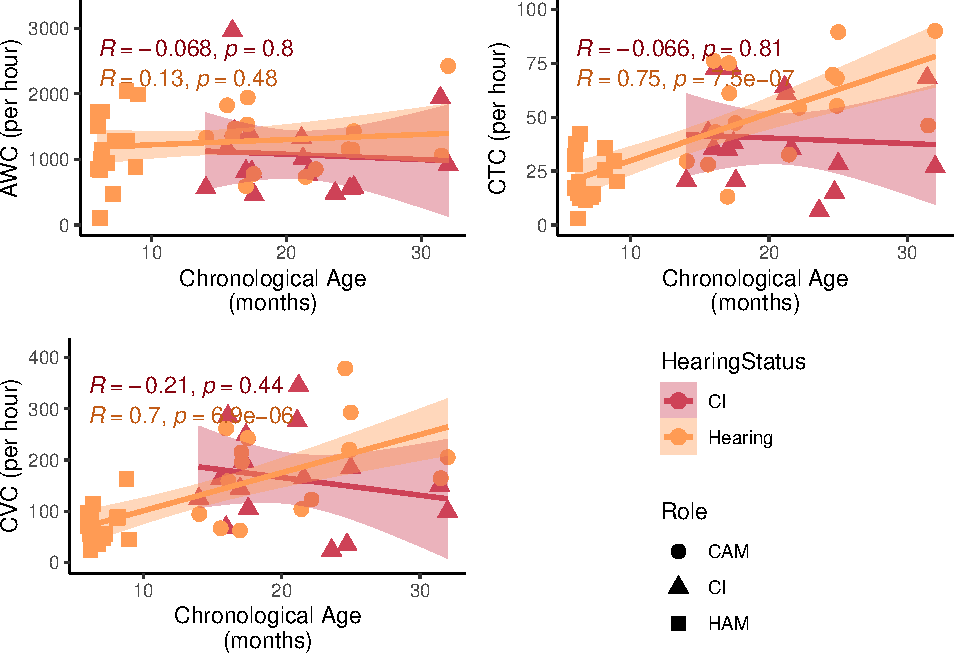
\includegraphics{DHH_Input_files/figure-latex/automated-plots-1.pdf}
\caption{\label{fig:automated-plots}Measures from Automated LENA analysis.}
\end{figure}

\subsubsection{Language Exposure Measures}\label{language-exposure-measures}

Total Word Count based on the manual annotations for each recording. This value is a count of all individual words produced by speakers other than the target child. Words were defined as strings separated by spaces in the transcription.

Each manually-coded utterance was annotated for its addressee: child, adult, both children and adults, a pet, other (e.g., virtual assistants, higher powers, themselves), or unknown addressee. While the annotation scheme does not distinguish speech directed to the target child from that directed to other children, looking at speech directed to adults, pets, and others allows for an estimation of the proportion of \emph{types} of speech each group is exposed to, (i.e., child directed speech vs.~overheard speech). We calculated the overall proportion of speech directed to each category.

To more closely estimate the overall quantity, we calculated these measures only in the 30 randomly-sampled minutes of transcription, not the 10 minutes selected for high-density talk.

\begin{figure}
\centering
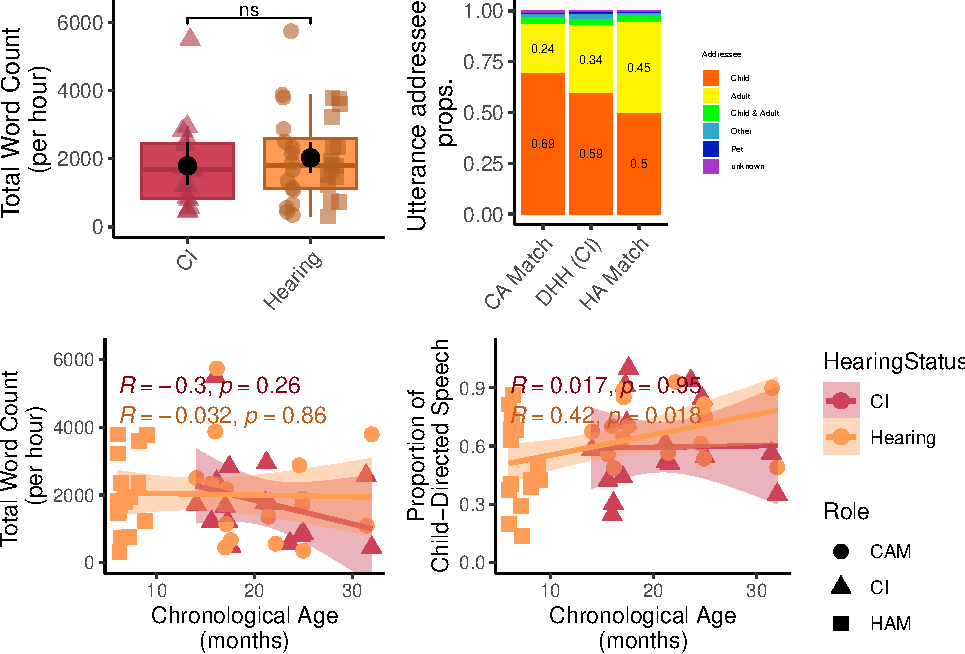
\includegraphics{DHH_Input_files/figure-latex/langex-plot-1.pdf}
\caption{\label{fig:langex-plot}Language exposure measures.}
\end{figure}

Language exposure was broadly quite similar between the CI group and each hearing match group. Because manual word count did not vary across age for typically-hearing participants (r = -0.03, \emph{p} = .861), we collapsed the CAM and HAM groups for the word count analysis. Results of the Wilcoxon test showed no significant difference in overall word count between the cochlear implant group and their typically-hearing matches (Mean\textsubscript{CI}=1793.38, Mean\textsubscript{Hearing}=2024.81, W = 227, \emph{p} = .537).

For the proportion of child-directed speech, we observed a significant correlation with age among the typically-hearing participants, so we ran a linear model with age and group as predictors (r = 0.42, \emph{p} = .018). This model does not significantly explain the variance in the proportion of child-directed speech (Model R² = 0.11, \emph{p} = .163, Beta\textsubscript{HearingStatus} = -0.13, \emph{p} = .558, Beta\textsubscript{Age} = 0, \emph{p} = .942, Interaction: Beta\textsubscript{HearingStatus:Age} = 0.01, \emph{p} = .371). Based on visual inspection of \ref{fig:langex-plot}, it seems like the proportion of child-directed speech might increase for typically-hearing children but not DHH children, but as seen in the graph, the proportion of child-directed speech shows wide individual variability, and our analysis does not yield any conclusions. statistical comparisons of other addressee proportions were not performed, as child-directed speech was the primary variable being investigated.

\subsubsection{Audibility Measures}\label{audibility-measures}

\begin{figure}
\centering
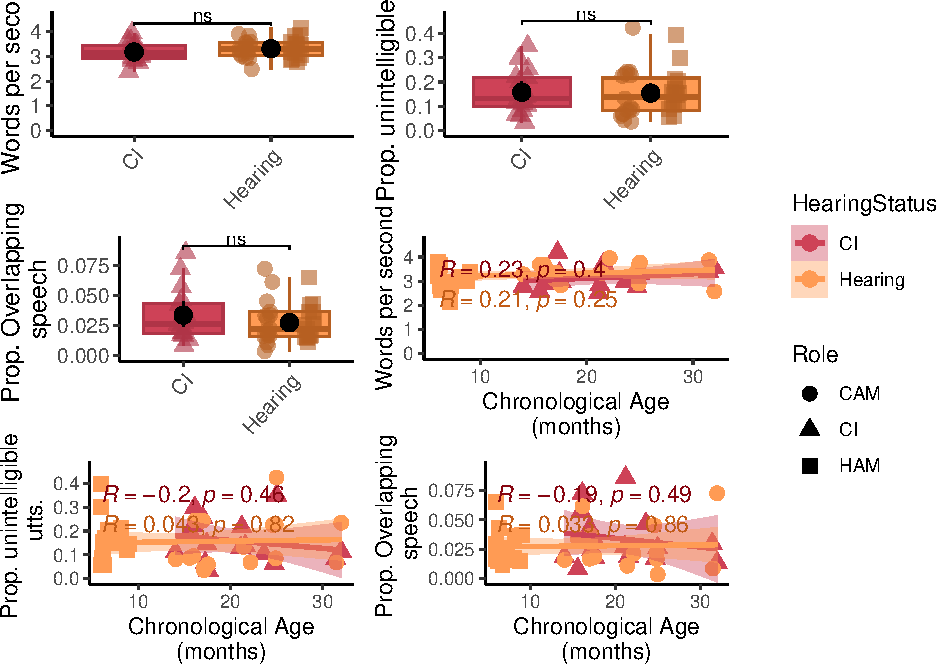
\includegraphics{DHH_Input_files/figure-latex/audibility-plot-1.pdf}
\caption{\label{fig:audibility-plot}Audibility measures.}
\end{figure}

In addition to automated audibility analyses, we computed three measures of input audibility based on the manual annotations. First, ``Words per Second'' measures the average rate of speech in the child's auditory environment. For each utterance, the number of words was divided by the duration of the utterance in seconds. These values were then averaged across all of the utterances in each recording. Utterances containing unintelligible speech were excluded from this calculation.

Second, we calculated the proportion of utterances containing speech deemed unintelligible. We note that this measure relied on the determination of intelligibility by an adult, typically-hearing listener listening to a recording and is thus an imperfect (though potentially still useful) proxy. That is, whether speech was or wasn't intelligible to the child cannot be captured, and this measure likely differs from the child's experience in several ways. First, though the child wore the recorder, the physical conditions of the the recorder differ from the child's own ears and cochlear implants (e.g.~could be muffled by their shirt when the child is being held). Second, for DHH children, we have no indicator of the acoustic quality of each utterance as it was processed through their cochlear implant. This measure is a proxy for identifying utterances that are far away, muffled, rapid, or obscured by competing sound and are more likely to be difficult for a language learner to process.

Finally, we calculated the proportion of overlapping speech in the manual transcription. Each utterance has an onset and offset time. When two or more utterances overlap in time, we count the overlapping duration towards the total amount of overlapping speech in the transcribed regions of the file. We report the proportion here as the summed duration of overlapping speech divided by the length of the recording.

Next, we investigated whether parents of children with cochlear implants might try to make speech more audible by slowing speech down (speech rate), speaking louder or more clearly (proportion of unintellible utterances), or reducing contexts where there are multiple speakers (proportion of overlapping utterances).

Because speech rate did not vary across age for typically-hearing participants (r = -0.09, \emph{p} = .625), we collapsed the CAM and HAM groups for the speech rate analysis. Results of the Wilcoxon test showed no significant difference in speech rate between the cochlear implant group and their typically-hearing matches (Mean\textsubscript{CI}=3.18, Mean\textsubscript{Hearing}=3.31, W = 210, \emph{p} = .323). The proportion of unintelligible utterances also did not vary across age for typically-hearing participants (r = 0.04, \emph{p} = .817), so we again collapsed the CAM and HAM groups for the proportion of unintelligible utterances analysis. Results of the Wilcoxon test showed no significant difference in proportion of unintelligible utterances between the cochlear implant group and their typically-hearing matches (Mean\textsubscript{CI}=0.16, Mean\textsubscript{Hearing}=0.15, W = 263, \emph{p} = .888).

Finally, since the proportion of overlapping utterances did not vary across age for typically-hearing participants (r = 0.03, \emph{p} = .857), we ran a Wilcoxon test comparing the amount of overlap in the input to typically-hearing children versus to children with cochlear implants. The two groups did not differ (Mean\textsubscript{CI}=0.03, Mean\textsubscript{Hearing}=0.03, W = 300, \emph{p} = .345).

\subsubsection{Complexity Measures}\label{complexity-measures}

We calculated Mean Length of Utterance, quantified as the mean number of morphemes per utterance in the speech input. Utterances' morpheme counts were parsed and counted using the \texttt{morphemepiece} package in R (Bratt, Harmon, \& Learning, 2022). We excluded utterances containing unintelligible speech.

We also calculated Type-Token Ratio to analyze the amount of lexical variety in each child's input. This measure was computed by ``chunking'' the input speech into 100-word bins across each group, then calculating the proportion of unique words out of the 100 in each bin. These uniqueness values were then averaged to produce a single value for Type-Token Ratio for each recording. Normalizing the denominator allows for a measure of lexical diversity that is less coupled with the raw quantity of speech in the input (Montag, Jones, \& Smith, 2018; \textbf{campbell2025?}).

\begin{figure}
\centering
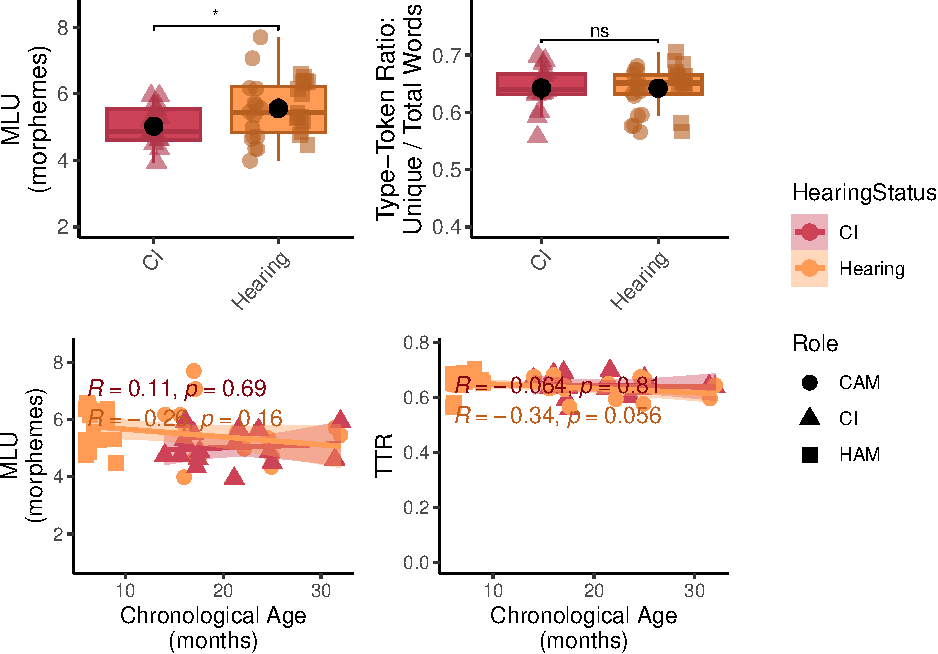
\includegraphics{DHH_Input_files/figure-latex/complexity-plot-1.pdf}
\caption{\label{fig:complexity-plot}Input complexity measures.}
\end{figure}

Neither MLU (r = -0.26, \emph{p} = .157) nor type-token ratio (r = -0.34, \emph{p} = .056) varied by age in the typically-hearing participants, so for both analyses, we collapsed the two typically-hearing subgroups. We found that MLU was higher for language input to typically-hearing infants (Mean\textsubscript{CI}=5.02, Mean\textsubscript{Hearing}=5.56, W = 160, \emph{p} = .036). Type-token ratio did not differ by group (Mean\textsubscript{CI}=0.64, Mean\textsubscript{Hearing}=0.64, W = 242, \emph{p} = .770).

\subsubsection{Conceptual Measures}\label{conceptual-measures}

We determined the temporality of each utterance following the procedure in (\textbf{campbell2025?}). To calculate this, we used the R package \texttt{udpipe} (\textbf{wijffels?}) to tag the first verb in each utterance with tense and mood features to determine the temporal quality of each utterance. Past tense, going to/want to/got to, and modal verbs were classified as decontextualized utterances, and present tense and gerunds were classified as present utterances. Fragments and other utterances for which no temporality features were tagged were left unclassified. For more discussion of the benefits and limitations of this analysis, see (\textbf{campbell2025?}).

\begin{figure}
\centering
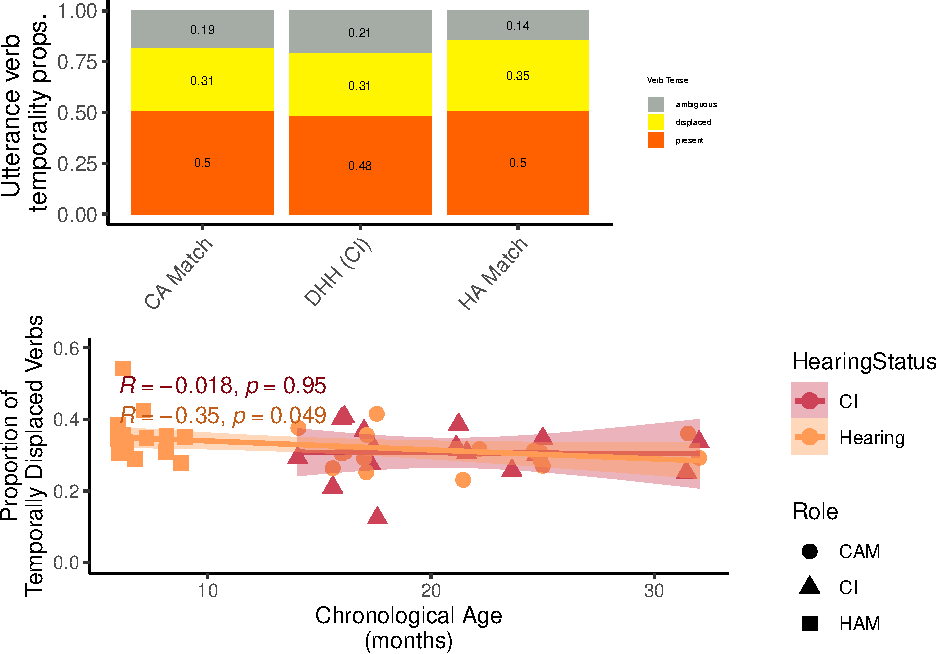
\includegraphics{DHH_Input_files/figure-latex/conceptual-plot-1.pdf}
\caption{\label{fig:conceptual-plot}Conceptual Measures.}
\end{figure}

Verb temporality did not differ across age for our typically-hearing participants (r = -0.13, \emph{p} = .478), so we collapsed the hearing groups together. Language input to the CI group contained a slightly lower proportion of temporally \emph{present} utterances (Mean\textsubscript{CI}=0.48, Mean\textsubscript{Hearing}=0.5, W = 163, \emph{p} = .042) but a similar amount of temporally displaced utterances (Mean\textsubscript{CI}=0.31, Mean\textsubscript{Hearing}=0.33, W = 222, \emph{p} = .468).

\subsubsection{Relationship between input and language outcomes}\label{relationship-between-input-and-language-outcomes}

We finally conducted two additional linear models, looking at both automated measures and measures from manually-annotated measures. For automated measures, we examined the effect of AWC on Child Vocalization Count, a numerical estimate expressed by the LENA software of the number of utterances produced by the child. For manual measures, we correlated Manual word Count and the proportion of the target child's utterances that were classified as canonical babbling (which includes lexical utterances).

\begin{figure}[h]
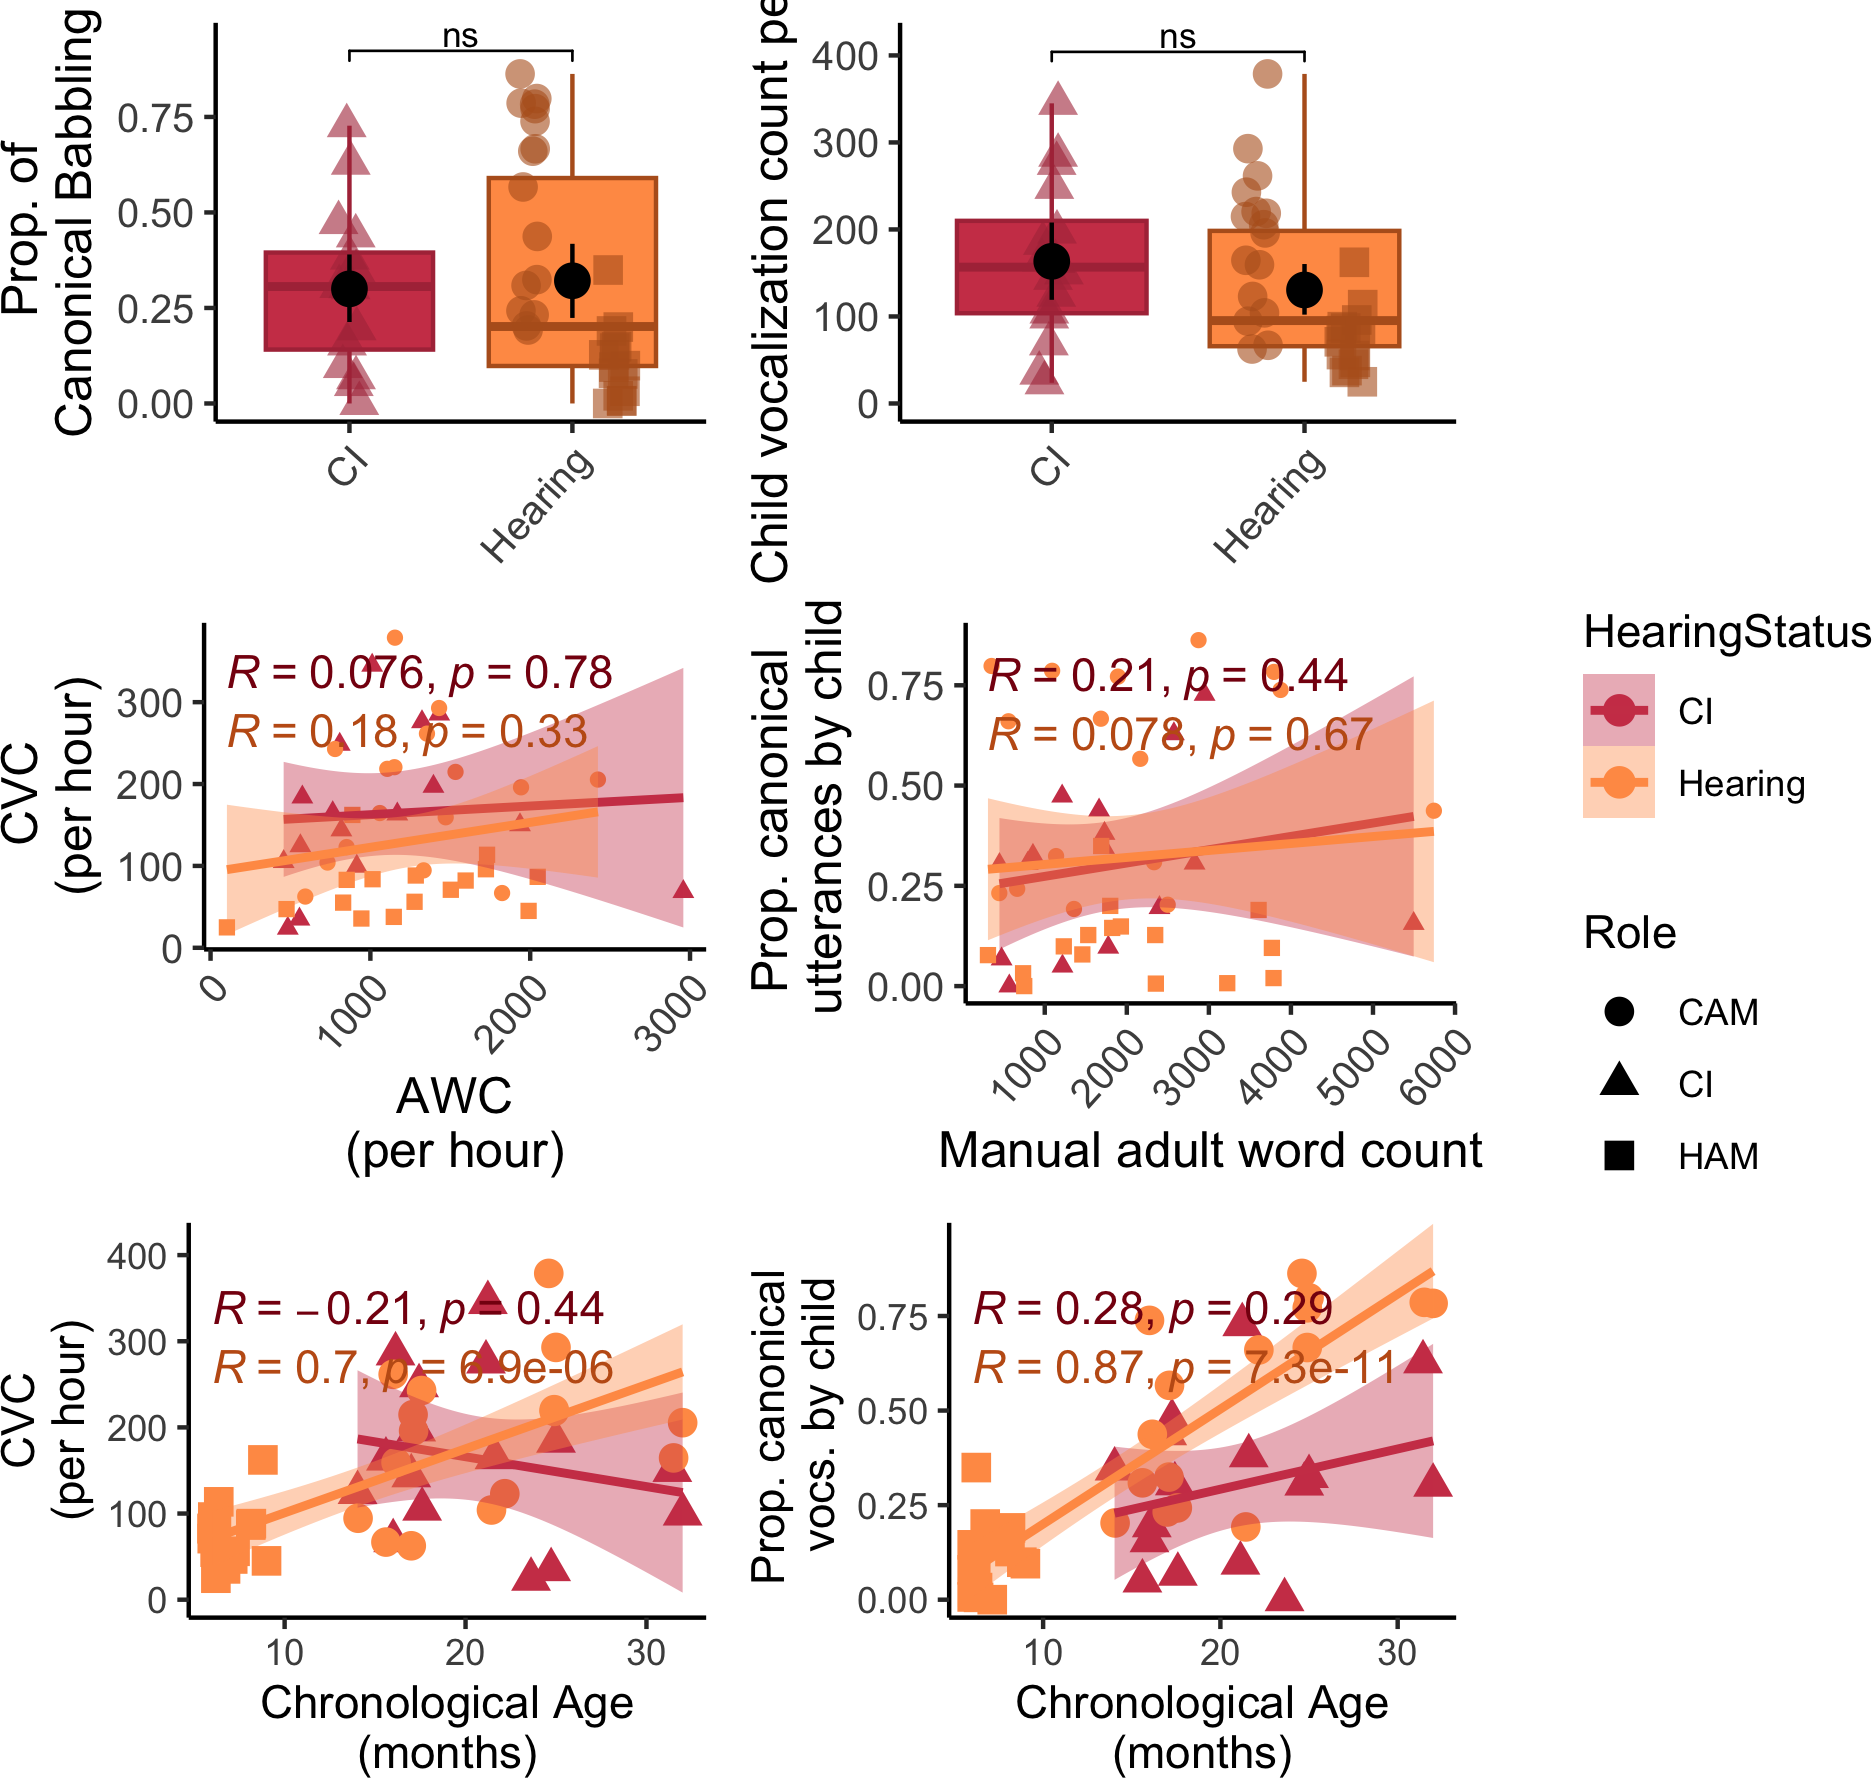
\includegraphics[height=1\textheight]{DHH_Input_files/figure-latex/chi-voc-plots-1} \caption{Input-Outcome relationships.}\label{fig:chi-voc-plots}
\end{figure}

Lastly, we measured whether characteristics of children's language \emph{input} predicted their language \emph{output}. We focused just on the relationship between parent input quantity and child input quantity / maturity, instead of testing each of the input variables above, but interested readers can access our data at OSF {[}link{]} and test other possible links. For this analysis, we created models predicting children's language productions, with main effects of Age, Hearing Status, and input variable, and an interaction between that input variable and hearing status.

We started by looking at Child Vocalization Count \textasciitilde{} Age + AdultWordCount\textsubscript{Manual} + HearingStatus + AdultWordCount\textsubscript{LENA}:HearingStatus. This model significantly predicted \textasciitilde18\% of the variance in child vocalization count (\emph{R}\textsuperscript{2}\textsubscript{adjusted} = 0.18, \emph{p} = .012). As expected, older children produced more vocalization counts (\emph{Beta} = 5.42, \emph{p} = .002), but we did not find significant effects of group (\emph{Beta} = -5.55, \emph{p} = .924), amount of adult words in the input (by the LENA automated count) (\emph{Beta} = 0.01, \emph{p} = .669), or the interaction between adult word count and group. (\emph{Beta} = 0.01, \emph{p} = .901).

Next, we analyzed whether the proportion of canonical utterances in the child's speech was predicted by Count \textasciitilde{} Age + AdultWordCount\textsubscript{Manual} + HearingStatus + AdultWordCount\textsubscript{Manual}:HearingStatus. This model significantly predicted \textasciitilde59\% of the variance in child vocalization count (\emph{R}\textsuperscript{2}\textsubscript{adjusted} = 0.59, \emph{p} \textless{} .001). As expected, older children produced more canonical utterances (\emph{Beta} = 0.03, \emph{p} \textless{} .001). We also observed that hearing children produced a higher proportion of canonical utterances (\emph{Beta} = 0.286, \emph{p} = .005), and children who were exposed to more words produced a higher proportion of canonical utterances (\emph{Beta} = 0.0001, \emph{p} = .047). We did not find an interaction between adult word count and group (\emph{Beta} = 0.000, \emph{p} = .271).

Lastly, we analyzed whether the proportion of \emph{lexical} utterances in the child's speech was predicted by Age + AdultWordCount\textsubscript{Manual} + HearingStatus + AdultWordCount\textsubscript{Manual}:HearingStatus. This model significantly predicted \textasciitilde67\% of the variance in child vocalization count (\emph{R}\textsuperscript{2}\textsubscript{adjusted} = 0.67, \emph{p} \textless{} .001). As expected, older children produced more lexical utterances (\emph{Beta} = 0.026, \emph{p} \textless{} .001). We also observed that hearing children produced a higher proportion of lexical utterances (\emph{Beta} = 0.36, \emph{p} \textless{} .001), and children who were exposed to more words produced a higher proportion of lexical utterances (\emph{Beta} = 0.0001, \emph{p} = .014). There was no interaction of adult word count and group (\emph{Beta} = -0.0001, \emph{p} = .073).

\phantomsection\label{refs}
\begin{CSLReferences}{1}{0}
\bibitem[\citeproctext]{ref-bratt2022}
Bratt, J., Harmon, J., \& Learning, B. F. \&. W. P. G. L. D. M. (2022). \emph{Morphemepiece: Morpheme tokenization}. Retrieved from \url{https://CRAN.R-project.org/package=morphemepiece}

\bibitem[\citeproctext]{ref-brugman2009}
Brugman, H., \& Russel, A. (2009). Annotating multimedia / multi-modal resources with ELAN. \emph{Proceedings of the Fourth International Conference on Language Resources and Evaluation}.

\bibitem[\citeproctext]{ref-ganek2016}
Ganek, H., \& Eriks-Brophy, A. (2016, November). \emph{The language ENvironment analysis (LENA) system: A literature review}. 2432. Umeå, Sweden: LiU Electronic Press. Retrieved from \url{https://aclanthology.org/W16-6504}

\bibitem[\citeproctext]{ref-gilkerson2008}
Gilkerson, J., \& Richards, J. (2008). \emph{The LENA natural language study}. Boulder, CO. Retrieved from \url{https://www.lena.org/wp-content/uploads/2016/07/LTR-02-2_Natural_Language_Study.pdf}

\bibitem[\citeproctext]{ref-lavechin}
Lavechin, M., Bousbib, R., Bredin, H., Dupoux, E., \& Cristia, A. (n.d.). \emph{An open-source voice type classifier for child-centered daylong recordings}. \url{https://doi.org/10.48550/arXiv.2005.12656}

\bibitem[\citeproctext]{ref-macwhinney2019}
MacWhinney, B. (2019). \emph{CHAT Manual}. \url{https://doi.org/10.21415/3MHN-0Z89}

\bibitem[\citeproctext]{ref-montag2018}
Montag, J. L., Jones, M. N., \& Smith, L. B. (2018). Quantity and Diversity: Simulating Early Word Learning Environments. \emph{Cognitive Science}, \emph{42 Suppl 2}(Suppl 2), 375--412. \url{https://doi.org/10.1111/cogs.12592}

\bibitem[\citeproctext]{ref-sloetjes2008}
Sloetjes, H., \& Wittenburg, P. (2008, May). \emph{Lrec 2008} (N. Calzolari, K. Choukri, B. Maegaard, J. Mariani, J. Odijk, S. Piperidis, \& D. Tapias, Eds.). Marrakech, Morocco: European Language Resources Association (ELRA). Retrieved from \url{http://www.lrec-conf.org/proceedings/lrec2008/pdf/208_paper.pdf}

\bibitem[\citeproctext]{ref-soderstrom2021}
Soderstrom, M., Casillas, M., Bergelson, E., Rosemberg, C., Alam, F., Warlaumont, A. S., \& Bunce, J. (2021). Developing a cross-cultural annotation system and MetaCorpus for studying infants{'} real world language experience. \emph{Collabra: Psychology}, \emph{7}(1), 23445. \url{https://doi.org/10.1525/collabra.23445}

\bibitem[\citeproctext]{ref-wang2022}
Wang, Y., Cooke, M., Reed, J., Dilley, L., \& Houston, D. (2022). Home auditory environments of children with cochlear implants and children with normal hearing. \emph{Ear and Hearing}, \emph{43}(2), 592. \url{https://doi.org/10.1097/AUD.0000000000001124}

\bibitem[\citeproctext]{ref-xu2009}
Xu, D., Yapanel, U., \& Gray, S. (2009). \emph{Reliability of the LENA language environment analysis system in young children{'}s natural home environment} (pp. 1--16). Boulder, CO. Retrieved from \url{https://www.lena.org/wp-content/uploads/2016/07/LTR-05-2_Reliability.pdf}

\bibitem[\citeproctext]{ref-zimmerman2009}
Zimmerman, F. J., Gilkerson, J., Richards, J., Christakis, D., Xu, D., Gray, S., \& Yapanel, U. (2009). Teaching by Listening: The Importance of Adult-Child Conversations to Language Development. \emph{Pediatrics}, \emph{124}(1), 342--349. \url{https://doi.org/10.1542/peds.2008-2267}

\end{CSLReferences}


\end{document}
